% Source of truth for the manuscript (replaces manuscript.md, 13 Nov 2026). Build: python3 paper/build.py
\documentclass[11pt]{article}
% Shared preamble of manuscript.tex and supplement.tex (built with tectonic; see paper/build.py)
\usepackage[a4paper,margin=2.5cm]{geometry}
\usepackage{fontspec}   % XeTeX (tectonic): Latin Modern OpenType by default, Unicode input
\usepackage{microtype}
\usepackage[running]{lineno}
\usepackage{graphicx}
\usepackage{booktabs}
\usepackage{longtable}
\usepackage{tabularx}
\usepackage{array}
\usepackage{caption}
\captionsetup{font=small,labelfont=bf,labelsep=period}
\usepackage{enumitem}
\setlist{itemsep=1pt,topsep=3pt}
\usepackage{amsmath}
\usepackage{xcolor}
\usepackage[numbers,sort&compress,square]{natbib}
\usepackage[hidelinks]{hyperref}
\urlstyle{same}
\setlength{\parskip}{3pt}
\renewcommand{\arraystretch}{1.15}
\newcolumntype{L}[1]{>{\raggedright\arraybackslash}p{#1}}
\newcolumntype{Y}{>{\raggedright\arraybackslash}X}

% Numbers: every number taken from the data is printed with \nm{key}; the values come from
% numbers.tex, which paper/make_numbers.py writes from the repository's files (sources in
% NUMBERS_generated.tsv, text-to-key map in NUMBERS.md). An unknown key stops the build.
\makeatletter
\newcommand{\nmdef}[2]{\expandafter\def\csname nm@#1\endcsname{#2}}
\newcommand{\nm}[1]{\ifcsname nm@#1\endcsname\csname nm@#1\endcsname\else\errmessage{unknown number key: #1}\fi}
\makeatother
% Generated by paper/make_numbers.py. Do not edit. Sources: paper/NUMBERS_generated.tsv
\nmdef{titin_len}{35,991}
\nmdef{pkz_len}{45,212}
\nmdef{uniprotkb_gt_titin}{51}
\nmdef{uniprotkb_gt_pkz}{4}
\nmdef{uniprotkb_pe3}{37}
\nmdef{uniprotkb_pe4}{14}
\nmdef{uniprotkb_reviewed}{0}
\nmdef{uniparc_gt_titin}{477}
\nmdef{uniparc_gt_pkz}{65}
\nmdef{ncbi_gt_titin}{472}
\nmdef{ncbi_gt_pkz}{47}
\nmdef{refseq_gt_titin}{349}
\nmdef{union_seqs}{552}
\nmdef{union_gt_pkz}{71}
\nmdef{union_live}{523}
\nmdef{excl_nolive}{29}
\nmdef{excl_patent}{6}
\nmdef{excl_partial}{7}
\nmdef{longest_record}{187,500}
\nmdef{n_retained}{510}
\nmdef{n_excluded}{42}
\nmdef{n_retained_gt_pkz}{57}
\nmdef{loci_retained_stage0}{228}
\nmdef{xp_records}{329}
\nmdef{xp_genes}{52}
\nmdef{n_euk}{452}
\nmdef{n_bact}{57}
\nmdef{n_arch}{1}
\nmdef{big_euk}{34}
\nmdef{big_bact}{23}
\nmdef{s1_all_A}{114}
\nmdef{s1_all_B}{213}
\nmdef{s1_all_C}{154}
\nmdef{s1_all_D}{29}
\nmdef{s1_big_A}{0}
\nmdef{s1_big_B}{4}
\nmdef{s1_big_C}{36}
\nmdef{s1_big_D}{17}
\nmdef{s2_all_A}{119}
\nmdef{s2_all_B}{267}
\nmdef{s2_all_C}{95}
\nmdef{s2_all_D}{29}
\nmdef{s2_big_A}{0}
\nmdef{s2_big_B}{5}
\nmdef{s2_big_C}{35}
\nmdef{s2_big_D}{17}
\nmdef{fin_all_A}{120}
\nmdef{fin_all_B}{267}
\nmdef{fin_all_C}{94}
\nmdef{fin_all_D}{29}
\nmdef{fin_big_A}{1}
\nmdef{fin_big_B}{5}
\nmdef{fin_big_C}{34}
\nmdef{fin_big_D}{17}
\nmdef{s1s2_C_to_B}{59}
\nmdef{s1s2_B_to_A}{5}
\nmdef{s1s2_C_to_B_apostichopus}{48}
\nmdef{rule_D1_all}{25}
\nmdef{rule_D1_big}{15}
\nmdef{rule_D2_all}{16}
\nmdef{rule_D2_big}{10}
\nmdef{rule_D3_all}{24}
\nmdef{rule_D3_big}{15}
\nmdef{rule_D5_all}{3}
\nmdef{rule_D5_big}{2}
\nmdef{rule_D1_big_euk}{14}
\nmdef{d1_pattern_all}{72}
\nmdef{d1_pattern_big}{32}
\nmdef{d1_pattern_big_euk}{29}
\nmdef{repeat_flag_all}{47}
\nmdef{repeat_flag_big}{17}
\nmdef{flag_big_weak_coding}{11}
\nmdef{flag_big_weak_coding_range}{0.919--0.942}
\nmdef{flag_big_coding}{4}
\nmdef{flag_big_nodna}{2}
\nmdef{d_big_d1_with_dna}{15}
\nmdef{d_big_d5}{2}
\nmdef{rna_not_tested_d1}{0}
\nmdef{rep_models}{43}
\nmdef{rep_testable}{10}
\nmdef{rep_testable_big}{5}
\nmdef{rep_jobs}{7}
\nmdef{rep_runs}{33}
\nmdef{rep_gb}{135}
\nmdef{rep_schisto1_supported}{32}
\nmdef{rep_schisto1_introns}{45}
\nmdef{rep_schisto1_testable}{32}
\nmdef{rep_schisto1_testable_unsup}{0}
\nmdef{rep_schisto1_unique_reads}{44,113}
\nmdef{rep_schisto1_verdict}{partial}
\nmdef{rep_schisto1_grade}{B}
\nmdef{rep_schisto2_supported}{32}
\nmdef{rep_schisto2_introns}{46}
\nmdef{rep_schisto2_testable}{32}
\nmdef{rep_schisto2_testable_unsup}{0}
\nmdef{rep_schisto2_unique_reads}{44,112}
\nmdef{rep_schisto2_verdict}{partial}
\nmdef{rep_schisto2_grade}{B}
\nmdef{rep_owenia_supported}{9}
\nmdef{rep_owenia_introns}{22}
\nmdef{rep_owenia_testable}{6}
\nmdef{rep_owenia_testable_unsup}{0}
\nmdef{rep_owenia_unique_reads}{673}
\nmdef{rep_owenia_verdict}{weak (unsupported introns lie where reads are too few)}
\nmdef{rep_owenia_grade}{C}
\nmdef{rep_arcto_supported}{1}
\nmdef{rep_arcto_introns}{7}
\nmdef{rep_arcto_testable}{0}
\nmdef{rep_arcto_testable_unsup}{0}
\nmdef{rep_arcto_unique_reads}{85}
\nmdef{rep_arcto_verdict}{weak (unsupported introns lie where reads are too few)}
\nmdef{rep_arcto_grade}{C}
\nmdef{rep_noexpr}{6}
\nmdef{rep_noexpr_max_unique}{34}
\nmdef{rep_contradicted}{0}
\nmdef{rep_to_B}{2}
\nmdef{rep_to_D}{0}
\nmdef{rep_run_results}{33}
\nmdef{rep_run_skips}{0}
\nmdef{rep_schisto_err10016938}{32}
\nmdef{mapp_gas1_uj}{25}
\nmdef{mapp_gas1_n}{2,053}
\nmdef{mapp_gas1_pct}{1}
\nmdef{mapp_gas2_uj}{26}
\nmdef{mapp_gas2_n}{1,273}
\nmdef{mapp_gas2_pct}{2}
\nmdef{mapp_gas3_uj}{27}
\nmdef{mapp_gas3_n}{1,208}
\nmdef{mapp_gas3_pct}{2}
\nmdef{mapp_acn_uj}{48}
\nmdef{mapp_acn_n}{1,035}
\nmdef{mapp_acn_pct}{5}
\nmdef{mapp_syn1_uj}{16}
\nmdef{mapp_syn1_n}{203}
\nmdef{mapp_syn1_pct}{8}
\nmdef{mapp_syn2_uj}{9}
\nmdef{mapp_syn2_n}{134}
\nmdef{mapp_syn2_pct}{7}
\nmdef{mapp_schisto1_uj}{37}
\nmdef{mapp_schisto1_n}{45}
\nmdef{mapp_schisto1_pct}{82}
\nmdef{mapp_owenia_uj}{22}
\nmdef{mapp_owenia_n}{22}
\nmdef{mapp_owenia_pct}{100}
\nmdef{mapp_arcto_uj}{7}
\nmdef{mapp_arcto_n}{7}
\nmdef{mapp_arcto_pct}{100}
\nmdef{ctl_release}{2026\_04}
\nmdef{ctl_n}{176}
\nmdef{ctl_silk_n}{3}
\nmdef{ctl_silk_d1}{1}
\nmdef{ctl_spidroin_n}{4}
\nmdef{ctl_spidroin_d1}{3}
\nmdef{ctl_mucin_n}{15}
\nmdef{ctl_mucin_d1}{0}
\nmdef{ctl_adhesin_n}{13}
\nmdef{ctl_adhesin_d1}{4}
\nmdef{ctl_long_n}{150}
\nmdef{ctl_long_d1}{3}
\nmdef{ctl_d1_flagged}{10}
\nmdef{ctl_d23_flagged}{0}
\nmdef{ctl_flagged_with_cds}{8}
\nmdef{ctl_flagged_fickett_min}{1.094}
\nmdef{ctl_flagged_open_max}{1}
\nmdef{hold_n}{9,428}
\nmdef{hold_trigger}{17}
\nmdef{hold_d1_v1}{17}
\nmdef{hold_d1_cds}{10}
\nmdef{hold_d1_v2}{0}
\nmdef{power_models}{57}
\nmdef{power_reps}{20}
\nmdef{power_shift_0.1_v1_contradicted}{0}
\nmdef{power_shift_0.1_v1_under-supported}{0}
\nmdef{power_shift_0.1_v1_partial}{0.997}
\nmdef{power_shift_0.1_v1_full}{0.003}
\nmdef{power_shift_0.1_v2_contradicted}{0}
\nmdef{power_shift_0.1_v2_under-supported}{0}
\nmdef{power_shift_0.1_v2_partial}{0.997}
\nmdef{power_shift_0.1_v2_full}{0.003}
\nmdef{power_shift_0.2_v1_contradicted}{0}
\nmdef{power_shift_0.2_v1_under-supported}{0}
\nmdef{power_shift_0.2_v1_partial}{1}
\nmdef{power_shift_0.2_v1_full}{0}
\nmdef{power_shift_0.2_v2_contradicted}{0}
\nmdef{power_shift_0.2_v2_under-supported}{0.865}
\nmdef{power_shift_0.2_v2_partial}{0.135}
\nmdef{power_shift_0.2_v2_full}{0}
\nmdef{power_shift_0.3_v1_contradicted}{0}
\nmdef{power_shift_0.3_v1_under-supported}{0}
\nmdef{power_shift_0.3_v1_partial}{1}
\nmdef{power_shift_0.3_v1_full}{0}
\nmdef{power_shift_0.3_v2_contradicted}{0}
\nmdef{power_shift_0.3_v2_under-supported}{1}
\nmdef{power_shift_0.3_v2_partial}{0}
\nmdef{power_shift_0.3_v2_full}{0}
\nmdef{power_shift_0.4_v1_contradicted}{0}
\nmdef{power_shift_0.4_v1_under-supported}{0}
\nmdef{power_shift_0.4_v1_partial}{1}
\nmdef{power_shift_0.4_v1_full}{0}
\nmdef{power_shift_0.4_v2_contradicted}{0}
\nmdef{power_shift_0.4_v2_under-supported}{1}
\nmdef{power_shift_0.4_v2_partial}{0}
\nmdef{power_shift_0.4_v2_full}{0}
\nmdef{power_shift_0.5_v1_contradicted}{0.725}
\nmdef{power_shift_0.5_v1_under-supported}{0.198}
\nmdef{power_shift_0.5_v1_partial}{0.076}
\nmdef{power_shift_0.5_v1_full}{0}
\nmdef{power_shift_0.5_v2_contradicted}{0.725}
\nmdef{power_shift_0.5_v2_under-supported}{0.275}
\nmdef{power_shift_0.5_v2_partial}{0}
\nmdef{power_shift_0.5_v2_full}{0}
\nmdef{power_shift_0.6_v1_contradicted}{1}
\nmdef{power_shift_0.6_v1_under-supported}{0}
\nmdef{power_shift_0.6_v1_partial}{0}
\nmdef{power_shift_0.6_v1_full}{0}
\nmdef{power_shift_0.6_v2_contradicted}{1}
\nmdef{power_shift_0.6_v2_under-supported}{0}
\nmdef{power_shift_0.6_v2_partial}{0}
\nmdef{power_shift_0.6_v2_full}{0}
\nmdef{power_skip_0.2_v1_contradicted}{0}
\nmdef{power_skip_0.2_v1_under-supported}{0}
\nmdef{power_skip_0.2_v1_partial}{1}
\nmdef{power_skip_0.2_v1_full}{0}
\nmdef{power_skip_0.2_v2_contradicted}{0}
\nmdef{power_skip_0.2_v2_under-supported}{0.278}
\nmdef{power_skip_0.2_v2_partial}{0.722}
\nmdef{power_skip_0.2_v2_full}{0}
\nmdef{power_skip_0.3_v1_contradicted}{0}
\nmdef{power_skip_0.3_v1_under-supported}{0}
\nmdef{power_skip_0.3_v1_partial}{1}
\nmdef{power_skip_0.3_v1_full}{0}
\nmdef{power_skip_0.3_v2_contradicted}{0}
\nmdef{power_skip_0.3_v2_under-supported}{1}
\nmdef{power_skip_0.3_v2_partial}{0}
\nmdef{power_skip_0.3_v2_full}{0}
\nmdef{power_skip_0.5_v1_contradicted}{0.242}
\nmdef{power_skip_0.5_v1_under-supported}{0.061}
\nmdef{power_skip_0.5_v1_partial}{0.696}
\nmdef{power_skip_0.5_v1_full}{0}
\nmdef{power_skip_0.5_v2_contradicted}{0.242}
\nmdef{power_skip_0.5_v2_under-supported}{0.758}
\nmdef{power_skip_0.5_v2_partial}{0}
\nmdef{power_skip_0.5_v2_full}{0}
\nmdef{power_skip_0.6_v1_contradicted}{0.981}
\nmdef{power_skip_0.6_v1_under-supported}{0.009}
\nmdef{power_skip_0.6_v1_partial}{0.011}
\nmdef{power_skip_0.6_v1_full}{0}
\nmdef{power_skip_0.6_v2_contradicted}{0.981}
\nmdef{power_skip_0.6_v2_under-supported}{0.019}
\nmdef{power_skip_0.6_v2_partial}{0}
\nmdef{power_skip_0.6_v2_full}{0}
\nmdef{pw_contr_ge60_min_pct}{98}
\nmdef{pw_shift50_pct}{73}
\nmdef{pw_skip50_pct}{24}
\nmdef{pw_v1_partial_2040_min_pct}{99.9}
\nmdef{pw_v2_down_3040_min_pct}{100}
\nmdef{pw_v2_shift20_pct}{87}
\nmdef{pw_v2_skip20_pct}{28}
\nmdef{pw_v2_10_down_pct}{0}
\nmdef{dnactl_v3_a_deletion_ill}{against: 1 single-copy boundary(ies) with 0 spanning pairs between well-covered windows; 1 clip pile-up(s) where physical coverage drops; discordant pairs up to 19\% in a window [0.66 kb in 1 stretch(es) where this library cannot place pairs uniquely (repeat), not crossed]}
\nmdef{dnactl_v3_a_deletion_illont}{against: 1 single-copy boundary(ies) with 0 spanning pairs between well-covered windows; 1 clip pile-up(s) where physical coverage drops; discordant pairs up to 19\% in a window [0.66 kb in 1 stretch(es) where this library cannot place pairs uniquely (repeat), not crossed]}
\nmdef{dnactl_v3_b_collapse_ill}{supported by the reads}
\nmdef{dnactl_v3_b_collapse_illont}{supported by the reads}
\nmdef{dnactl_v3_c_expansion_ill}{supported outside 9.37 kb of repeat (no long reads to resolve it)}
\nmdef{dnactl_v3_c_expansion_illont}{supported outside 9.37 kb of repeat; long reads do not span it}
\nmdef{dnactl_v3_d_rrna_correct_ill}{supported outside 4.89 kb of repeat (no long reads to resolve it)}
\nmdef{dnactl_v3_d_rrna_correct_illont}{supported by the reads (short reads; the 4.89 kb repeat block(s) spanned by 13+ long reads)}
\nmdef{dnactl_v3_e_segdup_correct_ill}{inconclusive: only 98.7\% of single-copy gene bases at depth $\geq$ 5 [12.0 kb in multi-copy block(s) that short reads cannot place; 13.04 kb in 4 stretch(es) where this library cannot place pairs uniquely (repeat), not crossed]}
\nmdef{dnactl_v3_e_segdup_correct_illont}{inconclusive: only 98.7\% of single-copy gene bases at depth $\geq$ 5 [12.0 kb in multi-copy block(s) that short reads cannot place; 13.04 kb in 4 stretch(es) where this library cannot place pairs uniquely (repeat), not crossed]}
\nmdef{dnactl_v31_a_deletion_ill}{against: 1 single-copy boundary(ies) with 0 spanning pairs between well-covered windows; 1 clip pile-up(s) where physical coverage drops; discordant pairs up to 19\% in a window [0.66 kb in 1 stretch(es) where this library cannot place pairs uniquely (repeat), not crossed]}
\nmdef{dnactl_v31_a_deletion_illont}{against: 1 single-copy boundary(ies) with 0 spanning pairs between well-covered windows; 1 clip pile-up(s) where physical coverage drops; discordant pairs up to 19\% in a window [0.66 kb in 1 stretch(es) where this library cannot place pairs uniquely (repeat), not crossed]}
\nmdef{dnactl_v31_b_collapse_ill}{against: copy-number anomaly (v3.1): 5 kb at 1.98x, excess copies (collapsed repeat?)}
\nmdef{dnactl_v31_b_collapse_ill_ratio}{1.98}
\nmdef{dnactl_v31_b_collapse_illont}{against: copy-number anomaly (v3.1): 5 kb at 1.98x, excess copies (collapsed repeat?)}
\nmdef{dnactl_v31_b_collapse_illont_ratio}{1.98}
\nmdef{dnactl_v31_c_expansion_ill}{against: copy-number anomaly (v3.1): 10 kb at 0.49x, deficit (expanded or absent?) [8.0 kb in multi-copy block(s) that short reads cannot place; 8.74 kb in 2 stretch(es) where this library cannot place pairs uniquely (repeat), not crossed]}
\nmdef{dnactl_v31_c_expansion_ill_ratio}{0.49}
\nmdef{dnactl_v31_c_expansion_illont}{against: copy-number anomaly (v3.1): 10 kb at 0.49x, deficit (expanded or absent?) [8.0 kb in multi-copy block(s) that short reads cannot place; 8.74 kb in 2 stretch(es) where this library cannot place pairs uniquely (repeat), not crossed]}
\nmdef{dnactl_v31_c_expansion_illont_ratio}{0.49}
\nmdef{dnactl_v31_d_rrna_correct_ill}{supported outside 4.89 kb of repeat (no long reads to resolve it)}
\nmdef{dnactl_v31_d_rrna_correct_illont}{supported by the reads (short reads; the 4.89 kb repeat block(s) spanned by 13+ long reads)}
\nmdef{dnactl_v31_e_segdup_correct_ill}{inconclusive: only 98.7\% of single-copy gene bases at depth $\geq$ 5 [12.0 kb in multi-copy block(s) that short reads cannot place; 13.04 kb in 4 stretch(es) where this library cannot place pairs uniquely (repeat), not crossed]}
\nmdef{dnactl_v31_e_segdup_correct_illont}{inconclusive: only 98.7\% of single-copy gene bases at depth $\geq$ 5 [12.0 kb in multi-copy block(s) that short reads cannot place; 13.04 kb in 4 stretch(es) where this library cannot place pairs uniquely (repeat), not crossed]}
\nmdef{dnactl_real_unchanged}{yes}
\nmdef{dnactl_repeat_depth_ratio_range}{0.84--0.97}
\nmdef{dnactl_omni_repeat_depth_ratio_range}{0.86--0.97}
\nmdef{sens_variants}{33}
\nmdef{sens_big_ab_stable}{31}
\nmdef{sens_big_ab_changed}{D3 open frames $\geq$ 1 (published 2), spliced reads per intron $\geq$ 10 (published 3)}
\nmdef{sens_s6_lenient_all_B}{267}
\nmdef{sens_base_all_B}{267}
\nmdef{sens_d1v1_big_D}{34}
\nmdef{sens_d1v1_all_D}{76}
\nmdef{sens_allA_range}{116--178}
\nmdef{dna_sens_settings}{7}
\nmdef{dna_sens_grade_changes}{min\_pairs\_per\_boundary=10}
\nmdef{prot_spectra}{594,284}
\nmdef{prot_db_entries}{151,457}
\nmdef{prot_fractions}{60}
\nmdef{prot_scan_share_pct}{48}
\nmdef{prot_id_rate_pct}{84.6}
\nmdef{prot_distal}{8,279, 12,982, 15,831, 16,949}
\nmdef{prot_psms}{502,718}
\nmdef{prot_decoy_psms}{5,026}
\nmdef{prot_peptides}{42,000}
\nmdef{prot_proteins}{7,981}
\nmdef{prot_giant_len}{39,686}
\nmdef{prot_giant_peptides}{186}
\nmdef{prot_giant_shared}{0}
\nmdef{prot_giant_psms}{1,487}
\nmdef{prot_giant_residues}{2,357}
\nmdef{prot_giant_cov_pct}{5.9}
\nmdef{prot_giant_regions}{86}
\nmdef{prot_giant_first}{292}
\nmdef{prot_giant_last_end}{16,957}
\nmdef{prot_giant_last_pct}{42.7}
\nmdef{prot_giant_fifths}{182, 3, 1, 0, 0}
\nmdef{prot_giant_first6000}{182}
\nmdef{prot_giant_after6000}{8,279, 12,982, 15,831, 16,949}
\nmdef{prot_giant_protein_q}{0.0002}
\nmdef{prot_rev_q}{0.063}
\nmdef{prot_shuf_q}{0.17}
\nmdef{prot_rev_psms}{0}
\nmdef{prot_shuf_psms}{0}
\nmdef{prot_tryptic_range}{41--63}
\nmdef{prot_repeat_span}{17,653--25,339}
\nmdef{prot_repeat_blocks}{5}
\nmdef{prot_peptides_in_or_after_repeats}{0}
\nmdef{prot_eftu_peptides}{23}
\nmdef{prot_eftu_cov_pct}{55}
\nmdef{prot_eftu_len}{400}
\nmdef{prot_l7_peptides}{6}
\nmdef{prot_l7_cov_pct}{68}
\nmdef{prot_l7_len}{128}
\nmdef{prot_top_n}{12}
\nmdef{prot_top_rank_giant}{11}
\nmdef{prot_top_cov_range}{40.8--78.3}
\nmdef{prot_wall_min}{35}
\nmdef{prot_rss_gb}{5.2}
\nmdef{raw_files}{60}
\nmdef{raw_conversion_errors}{0}
\nmdef{raw_ms2}{1,106,517}
\nmdef{raw_mgf_share_pct}{54}
\nmdef{raw_instrument}{Orbitrap Velos Pro}
\nmdef{raw_psms}{507,612}
\nmdef{raw_peptides}{40,845}
\nmdef{raw_proteins}{7,560}
\nmdef{raw_giant_peptides}{182}
\nmdef{raw_giant_psms}{1,505}
\nmdef{raw_giant_residues}{2,282}
\nmdef{raw_giant_cov_pct}{5.8}
\nmdef{raw_giant_fifths}{179, 3, 0, 0, 0}
\nmdef{raw_giant_first6000}{179}
\nmdef{raw_giant_after6000}{8,279, 12,982, 15,831}
\nmdef{raw_giant_last_end}{15,840}
\nmdef{raw_giant_last_pct}{39.9}
\nmdef{raw_giant_protein_q}{0.00022}
\nmdef{raw_rev_q}{0.089}
\nmdef{raw_shuf_q}{0.17}
\nmdef{raw_rev_psms}{0}
\nmdef{raw_shuf_psms}{0}
\nmdef{raw_eftu_peptides}{24}
\nmdef{raw_eftu_cov_pct}{57}
\nmdef{raw_l7_peptides}{5}
\nmdef{raw_l7_cov_pct}{56}
\nmdef{raw_both}{179}
\nmdef{raw_only_raw}{3}
\nmdef{raw_only_mgf}{7}
\nmdef{raw_mgf_only_after6000}{16,949}
\nmdef{raw_in_or_after_repeats}{0}
\nmdef{raw_wall_min}{56}
\nmdef{prot_peak_last_q}{0.0096}
\nmdef{sy_ms2}{131,021}
\nmdef{sy_raw_files}{5}
\nmdef{sy_db_kept}{99,767}
\nmdef{sy_db_authors}{99,773}
\nmdef{sy_fragments}{6}
\nmdef{sy_fragment_max_len}{46,359}
\nmdef{sy_psms_spec}{272}
\nmdef{sy_peptides_spec}{88}
\nmdef{sy_min_pep_q}{0.018}
\nmdef{sy_min_prot_q}{0.024}
\nmdef{sy_authors_n}{37}
\nmdef{sy_authors_found}{31}
\nmdef{sy_giant_psms_spec}{0}
\nmdef{sy_giant_psms_any}{17}
\nmdef{sy_rev_psms_any}{27}
\nmdef{sy_shuf_psms_any}{15}
\nmdef{sy_calc3_psms}{30}
\nmdef{sy_tub_psms}{37}
\nmdef{sy_ef2_psms}{9}
\nmdef{prot_authors_file}{Mudpit\_160213\_OV3\_P5\_SK\_JHa\_372-Pe1\_01.mzid.gz}
\nmdef{prot_authors_len}{39,671}
\nmdef{prot_authors_peptides}{174}
\nmdef{prot_authors_fifths}{130, 2, 2, 2, 0}
\nmdef{prot_authors_last_start}{25,870}
\nmdef{prot_authors_pass_peptides}{130}
\nmdef{prot_authors_pass_fifths}{101, 0, 0, 0, 0}
\nmdef{pride_omni}{0}
\nmdef{pride_noc881}{0}
\nmdef{pride_noc1730}{0}
\nmdef{pride_sycon}{2}
\nmdef{pride_velam}{1}
\nmdef{prot_raw_files}{60}
\nmdef{prot_raw_gb}{15.3}
\nmdef{prot_closed_genome_proteins}{1,863}
\nmdef{raw_giant_last_pct_round}{40}
\nmdef{rep_untestable_noruns}{28}
\nmdef{rep_untestable_nolocus}{5}
\nmdef{twin_fix_n}{6}
\nmdef{twin_fix_big}{0}
\nmdef{rep_noruns_plectranthus}{25}
\nmdef{rep_noruns_merlangius}{2}
\nmdef{rep_noruns_coilia}{1}
\nmdef{raw_giant_unc_pct}{60}
\nmdef{prot_giant_grade}{C}
\nmdef{lb_loci}{213}
\nmdef{lb_excluded_rows}{42}
\nmdef{lb_A}{9}
\nmdef{lb_B}{85}
\nmdef{lb_C}{90}
\nmdef{lb_D}{29}
\nmdef{lb_big}{55}
\nmdef{lb_big_A}{1}
\nmdef{lb_big_B}{3}
\nmdef{lb_big_C}{34}
\nmdef{lb_big_D}{17}
\nmdef{lb_merged_records}{11}
\nmdef{lb_A_titin_loci}{8}
\nmdef{lb_A_titin_min}{36,247}
\nmdef{lb_A_titin_max}{38,490}
\nmdef{rna_runs_total}{269}
\nmdef{rna_runs_kept}{261}
\nmdef{rna_runs_superseded}{8}
\nmdef{rna_runs_followup}{16}
\nmdef{rna_species}{71}
\nmdef{rna_runs_v1}{8}
\nmdef{rna_runs_v2}{253}
\nmdef{rna_reads_billion}{11.6}
\nmdef{rna_runs_stream_error}{51}
\nmdef{rna_runs_stream_error_first}{46}
\nmdef{rna_stream_error_frac_median_pct}{68}
\nmdef{rna_stream_error_frac_min_pct}{9}
\nmdef{rna_runs_saturation}{55}
\nmdef{rna_runs_readcap}{20}
\nmdef{rna_frac_read_median_pct}{88}
\nmdef{rna_runs_lt50}{49}
\nmdef{rna_full}{59}
\nmdef{rna_partial}{75}
\nmdef{rna_weak}{27}
\nmdef{rna_noexpr}{12}
\nmdef{rna_noruns}{127}
\nmdef{rna_nottested}{15}
\nmdef{rna_notselected}{137}
\nmdef{rna_prok}{58}
\nmdef{rna_contradicted}{0}
\nmdef{rna_tested_models}{173}
\nmdef{titin_runs}{6}
\nmdef{titin_reads_unique}{361,467}
\nmdef{titin_n_introns}{361}
\nmdef{titin_introns_unique_support}{340}
\nmdef{titin_introns_multi_only}{13}
\nmdef{titin_introns_counted_supported}{353}
\nmdef{titin_cds_breadth}{0.973}
\nmdef{titin_testable_introns}{325}
\nmdef{titin_testable_introns_unsupported}{0}
\nmdef{pkz_runs}{7}
\nmdef{pkz_reads_unique}{71,183}
\nmdef{pkz_n_introns}{16}
\nmdef{pkz_introns_unique_support}{9}
\nmdef{pkz_introns_multi_only}{7}
\nmdef{pkz_introns_counted_supported}{16}
\nmdef{pkz_cds_breadth}{0.733}
\nmdef{pkz_testable_introns}{12}
\nmdef{pkz_testable_introns_unsupported}{0}
\nmdef{sycon_runs}{6}
\nmdef{sycon_reads_unique}{49,375}
\nmdef{sycon_n_introns}{24}
\nmdef{sycon_introns_unique_support}{22}
\nmdef{sycon_introns_multi_only}{0}
\nmdef{sycon_introns_counted_supported}{22}
\nmdef{sycon_cds_breadth}{1.0}
\nmdef{sycon_testable_introns}{24}
\nmdef{sycon_testable_introns_unsupported}{2}
\nmdef{halichondria_runs}{4}
\nmdef{halichondria_reads_unique}{70,304}
\nmdef{halichondria_n_introns}{2}
\nmdef{halichondria_introns_unique_support}{2}
\nmdef{halichondria_introns_multi_only}{0}
\nmdef{halichondria_introns_counted_supported}{2}
\nmdef{halichondria_cds_breadth}{0.979}
\nmdef{halichondria_testable_introns}{0}
\nmdef{halichondria_testable_introns_unsupported}{0}
\nmdef{titin_introns_none}{8}
\nmdef{microcaecilia_testable}{41}
\nmdef{microcaecilia_testable_unsup}{1}
\nmdef{microcaecilia_verdict}{partial}
\nmdef{rana_testable}{63}
\nmdef{rana_testable_unsup}{1}
\nmdef{rana_verdict}{partial}
\nmdef{solea_testable}{57}
\nmdef{solea_testable_unsup}{1}
\nmdef{solea_verdict}{partial}
\nmdef{pantherophis_testable}{21}
\nmdef{pantherophis_testable_unsup}{0}
\nmdef{pantherophis_verdict}{weak (unsupported introns lie where reads are too few)}
\nmdef{liftover_moved}{143}
\nmdef{liftover_n_introns}{334}
\nmdef{cam_after_sup}{67}
\nmdef{cam_after_testable_unsup}{0}
\nmdef{ovis_length}{98,182}
\nmdef{ovis_n_exons}{37}
\nmdef{ovis_genomic_span_bp}{356,419}
\nmdef{ovis_protein_period_aa}{22}
\nmdef{ovis_protein_period_identity}{0.847}
\nmdef{ovis_rep25_frac}{0.9922}
\nmdef{ovis_gc_cds}{0.678}
\nmdef{ovis_dna_tandem_lag_bp}{22}
\nmdef{ovis_dna_tandem_identity}{0.939}
\nmdef{ovis_fickett_median}{0.465}
\nmdef{ovis_n_other_frames_open}{2}
\nmdef{ovis_min_stops_per_kcodon_other_frames}{1.2}
\nmdef{ovis_rna_reads}{50,777,537}
\nmdef{ovis_rna_candidates}{0}
\nmdef{ovis_period22_entries}{10}
\nmdef{cirrhinus_len}{59,714}
\nmdef{cirrhinus_exons}{454}
\nmdef{cirrhinus_runs}{6}
\nmdef{cirrhinus_reads_unique}{54,161}
\nmdef{cirrhinus_n_introns}{453}
\nmdef{cirrhinus_introns_counted_supported}{356}
\nmdef{bagarius_len}{54,498}
\nmdef{bagarius_exons}{417}
\nmdef{bagarius_runs}{2}
\nmdef{bagarius_reads_unique}{4,277}
\nmdef{bagarius_n_introns}{416}
\nmdef{bagarius_introns_counted_supported}{144}
\nmdef{cirrhinus_second_copy_start_aa}{31,001}
\nmdef{cirrhinus_first_ttna}{30 of 30}
\nmdef{cirrhinus_second_ttnb}{20 of 29}
\nmdef{bagarius_second_copy_start_aa}{32,001}
\nmdef{bagarius_first_ttna}{31 of 31}
\nmdef{bagarius_second_ttnb}{11 of 22}
\nmdef{cirrhinus_join_intron_aa}{30,675}
\nmdef{cirrhinus_join_intron_reads}{0}
\nmdef{cirrhinus_join_before_median}{103}
\nmdef{cirrhinus_join_after_median}{2}
\nmdef{ovis_entries}{11}
\nmdef{ovis_period_multiple22}{11}
\nmdef{sycon_gap_patch_bp}{2,968}
\nmdef{sycon_best_homolog_len}{4,063}
\nmdef{sycon_len}{50,516}
\nmdef{nbc00881_len}{59,275}
\nmdef{nbc00881_ratio}{1.27}
\nmdef{nbc00881_best_len}{46,734}
\nmdef{nbc00881_orf_bp}{177,828}
\nmdef{nbc01730_len}{51,778}
\nmdef{nbc01730_ratio}{1.11}
\nmdef{nbc01730_best_len}{46,734}
\nmdef{nbc01730_orf_bp}{155,337}
\nmdef{pkz_uniprot_pe}{Predicted}
\nmdef{stage1_cpu_hours}{4.4}
\nmdef{ovis_stops_six_frames}{0, 1.2, 1.2, 45.6, 45.2, 45.5}
\nmdef{dna_oub_reads}{83,321,080}
\nmdef{dna_oub_reads_expected}{83,321,080}
\nmdef{dna_oub_depth}{45}
\nmdef{dna_oub_ratio}{1.12}
\nmdef{dna_oub_span_median}{38}
\nmdef{dna_oub_span_min_testable}{4}
\nmdef{dna_oub_discordant_pct}{1.5}
\nmdef{dna_oub_insert}{288}
\nmdef{dna_oub_untestable}{1}
\nmdef{dna_oub_boundaries}{257}
\nmdef{dna_oub_verdict}{inconclusive: weakest single-copy boundary spanned by 4 [1.34 kb in 2 stretch(es) where this library cannot place pairs uniquely (repeat), not crossed]}
\nmdef{dna_oub_control}{yes}
\nmdef{dna_oub_v2}{against: 1 single-copy boundary(ies) with 0 spanning pairs between well-covered windows}
\nmdef{dna_oub_E_at_untestable}{0}
\nmdef{dna_oub_obs_at_untestable}{0}
\nmdef{dna_oub_weakest}{4--5.8}
\nmdef{dna_nbc00881_reads}{14,056,286}
\nmdef{dna_nbc00881_reads_expected}{14,056,286}
\nmdef{dna_nbc00881_depth}{252}
\nmdef{dna_nbc00881_ratio}{1.02}
\nmdef{dna_nbc00881_span_median}{252}
\nmdef{dna_nbc00881_span_min_testable}{159}
\nmdef{dna_nbc00881_discordant_pct}{1.2}
\nmdef{dna_nbc00881_insert}{340}
\nmdef{dna_nbc00881_untestable}{1}
\nmdef{dna_nbc00881_boundaries}{177}
\nmdef{dna_nbc00881_verdict}{supported by the reads (short reads; the 1.1 kb repeat block(s) spanned by 64+ long reads)}
\nmdef{dna_nbc00881_control}{yes}
\nmdef{dna_nbc00881_v2}{supported by the reads}
\nmdef{dna_nbc00881_E_at_untestable}{0}
\nmdef{dna_nbc00881_obs_at_untestable}{6}
\nmdef{dna_nbc00881_weakest}{159--163}
\nmdef{dna_nbc00881_ont_reads}{61,843}
\nmdef{dna_nbc00881_ont_span_blocks}{64--67}
\nmdef{dna_nbc01730_reads}{15,565,314}
\nmdef{dna_nbc01730_reads_expected}{15,565,314}
\nmdef{dna_nbc01730_depth}{272}
\nmdef{dna_nbc01730_ratio}{1.02}
\nmdef{dna_nbc01730_span_median}{284}
\nmdef{dna_nbc01730_span_min_testable}{74}
\nmdef{dna_nbc01730_discordant_pct}{1.4}
\nmdef{dna_nbc01730_insert}{347}
\nmdef{dna_nbc01730_untestable}{8}
\nmdef{dna_nbc01730_boundaries}{155}
\nmdef{dna_nbc01730_verdict}{supported by the reads (short reads; the 9.0 kb repeat block(s) spanned by 9+ long reads)}
\nmdef{dna_nbc01730_control}{yes}
\nmdef{dna_nbc01730_v2}{supported by the reads (short reads; the 9.0 kb repeat block(s) spanned by 9+ long reads)}
\nmdef{dna_nbc01730_E_at_untestable}{0, 0, 0, 0, 0, 0, 0, 0}
\nmdef{dna_nbc01730_obs_at_untestable}{0, 0, 0, 0, 0, 0, 0, 0}
\nmdef{dna_nbc01730_weakest}{74--22.2}
\nmdef{dna_nbc01730_ont_reads}{36,579}
\nmdef{dna_nbc01730_ont_span_blocks}{9}
\nmdef{dna_tdt_reads}{85,214,796}
\nmdef{dna_tdt_reads_expected}{85,214,796}
\nmdef{dna_tdt_depth}{40}
\nmdef{dna_tdt_ratio}{1.08}
\nmdef{dna_tdt_span_median}{34}
\nmdef{dna_tdt_span_min_testable}{14}
\nmdef{dna_tdt_discordant_pct}{2.1}
\nmdef{dna_tdt_insert}{295}
\nmdef{dna_tdt_untestable}{1}
\nmdef{dna_tdt_boundaries}{257}
\nmdef{dna_tdt_verdict}{supported outside 1.32 kb of repeat (no long reads to resolve it)}
\nmdef{dna_tdt_control}{yes}
\nmdef{dna_tdt_v2}{n/a (judged under v3 only)}
\nmdef{dna_tdt_E_at_untestable}{0}
\nmdef{dna_tdt_obs_at_untestable}{0}
\nmdef{dna_tdt_weakest}{14--19.1}
\nmdef{dna_pmg_reads}{78,636,086}
\nmdef{dna_pmg_reads_expected}{78,636,086}
\nmdef{dna_pmg_depth}{52}
\nmdef{dna_pmg_ratio}{1.06}
\nmdef{dna_pmg_span_median}{45}
\nmdef{dna_pmg_span_min_testable}{15}
\nmdef{dna_pmg_discordant_pct}{1.9}
\nmdef{dna_pmg_insert}{292}
\nmdef{dna_pmg_untestable}{1}
\nmdef{dna_pmg_boundaries}{257}
\nmdef{dna_pmg_verdict}{supported outside 1.3 kb of repeat (no long reads to resolve it)}
\nmdef{dna_pmg_control}{yes}
\nmdef{dna_pmg_v2}{against: 1 single-copy boundary(ies) with 0 spanning pairs between well-covered windows}
\nmdef{dna_pmg_E_at_untestable}{0}
\nmdef{dna_pmg_obs_at_untestable}{0}
\nmdef{dna_pmg_weakest}{15--43.6}
\nmdef{orf_bp}{257,412}
\nmdef{contig_len_tdt}{1,614,705}
\nmdef{rep_lag_bp}{10,362}
\nmdef{rep_lag_codons}{3,454}
\nmdef{rep_copy_bp}{1,184}
\nmdef{rep_copy_a}{223,454--224,637}
\nmdef{rep_copy_b}{233,816--234,999}
\nmdef{rep_diffs}{2}
\nmdef{orf_len_aa}{85,803}
\nmdef{rep_copy_bp_kb}{1.18}
\nmdef{dna_oub_weakest_obs}{4}
\nmdef{dna_oub_weakest_exp}{6}
\nmdef{orf_len_if_excised}{82,349}
\nmdef{omni_copies}{3}
\nmdef{omni_aa_identity_min_pct}{99.96}
\nmdef{omni_aa_identity_max_pct}{99.98}
\nmdef{omni_contig_lengths}{1,614,705, 1,613,271, 1,168,148}
\nmdef{omni_n_in_cds}{0}
\nmdef{hmm_panel}{74}
\nmdef{s2_A_titin}{119}
\nmdef{s1_fix_B_to_C}{48}
\nmdef{titin_downgrades_withdrawn}{5}
\nmdef{cirrhinus_first_end}{31,000}


\newcommand{\gene}[1]{\textit{#1}}
\newcommand{\spn}[1]{\textit{#1}}
\newcommand{\Ca}{\textit{Candidatus}}
\newcommand{\placeholder}[1]{\textcolor{red!70!black}{[#1]}}
% table bodies from paper/tables are read with the primitive \input (LaTeX's \input breaks \bottomrule)
\makeatletter\newcommand{\tablebody}[1]{\@@input #1 }\makeatother
\newcommand{\file}[1]{\texttt{\detokenize{#1}}}

\title{Evidence grades for protein database entries longer than titin}
\author{Ahmet Tahir Mat\\[2pt]\small Papex Labs\\[2pt]\small Correspondence: \href{mailto:ahmet@papex.org}{ahmet@papex.org}}
\date{\small 13 November 2026. Preprint, not peer reviewed.}

\begin{document}
\maketitle

\begin{abstract}
\noindent Protein databases hold hundreds of sequences longer than titin, the muscle protein often described as the largest
protein. Most are gene predictions whose records do not state their evidence. We collected every sequence longer
than a \nm{titin_len}-aa human titin isoform from UniProtKB, UniParc and NCBI Protein and kept \nm{n_retained};
\nm{n_retained_gt_pkz} are longer than PKZILLA-1 (\nm{pkz_len} aa). Each was graded A--D by explicit checks, then tested
with public RNA-seq (\nm{rna_runs_kept} runs) or, for three bacterial models, with their source reads. Of the
\nm{n_retained_gt_pkz}, \nm{fin_big_D} are contradicted (grade D) and \nm{fin_big_C} have no line of support (C). The
most common pattern, a translated tandem DNA repeat, also marks real silk proteins and adhesins in our positive controls,
so it counts against a model only with DNA-level evidence; RNA-seq can rarely settle these models, because almost none of
their splice junctions is unique. Two fish models are consistent with merged tandem titin genes. Six sequences, at four
loci, reach grade A or B, all on gene-model evidence and stable in \nm{sens_big_ab_stable} of \nm{sens_variants}
threshold settings; the longest, an \nm{orf_len_aa}-aa \Ca{} Omnitrophota open reading frame, is supported by its source
reads except across a 1.2-kb repeat. For a \nm{prot_giant_len}-aa \Ca{} Velamenicoccus protein whose detection its
authors had reported, all \nm{raw_files} raw proteomics files gave \nm{raw_giant_peptides} unique peptides, none beyond
its first \nm{raw_giant_last_pct_round}\,\%: the N-terminal part is made, a full-length chain is not shown. Controls
exposed weaknesses in three of our rules; we report every revision and release the table, rules and code.
\end{abstract}

\section{Introduction}

Titin, the giant protein of striated muscle, is often described as the largest protein \citep{labeit1995,westroberts2023};
its complete gene sequence is known \citep{bang2001}. Human titin isoforms reach \nm{titin_len} aa (RefSeq
NP\_001254479.2), the length we use as the threshold here. In 2024, \citet{fallon2024} described PKZILLA-1, a polyketide
synthase of the haptophyte \spn{Prymnesium parvum} of \nm{pkz_len} aa, supported by RNA-seq across the gene and by
peptides that map uniquely to 7 of its 17 exons. \citet{westroberts2023} used genome curation of metagenome assemblies to
recover predicted proteins of up to 85,804 aa, most common in \Ca{} Omnitrophota; their preprint has no journal version
listed.

Protein databases hold many more entries of this size. \citet{amaral2024} surveyed more than 41,000 UniProtKB proteins
of at least 5,000 aa and discussed indirect indicators of whether such ``huge proteins'' are real. Giant genes in bacteria
have long been described \citep{reva2008}, and gene-model errors that merge neighbouring genes remain common in
eukaryotic annotations \citep{bachler2025}. Tools such as GeneValidator \citep{dragan2016} and OMArk \citep{nevers2025}
assess gene models one gene or one proteome at a time.

We did not find a per-entry account of the longest database entries: which are supported as full-length gene models,
which are contradicted, and by what evidence. We therefore graded every sequence longer than \nm{titin_len} aa in three
databases with explicit, rerunnable checks; reanalysed public RNA-seq for the eukaryotic models; re-mapped the original
sequencing reads for three bacterial models; and re-searched public proteomics data where they exist for an entry or its
organism. The result is an evidence-graded table. It is not a claim of a new longest protein, and none of the entries we
grade is newly described here.

\section{Results}

\subsection{An inventory of \nm{union_seqs} sequences longer than titin}

UniProtKB (release 2026\_04) holds \nm{uniprotkb_gt_titin} entries longer than \nm{titin_len} aa, UniParc
\nm{uniparc_gt_titin} and NCBI Protein (11 November 2026) \nm{ncbi_gt_titin} records, \nm{refseq_gt_titin} of them RefSeq
(Table~\ref{tab:inventory}). None of the UniProtKB entries is reviewed; their evidence levels are ``inferred from
homology'' (\nm{uniprotkb_pe3}) and ``predicted'' (\nm{uniprotkb_pe4}), as is PKZILLA-1's own entry (A0AB34IYJ6).
The union holds \nm{union_seqs} unique sequences (merged by MD5 checksum), \nm{union_gt_pkz} of them longer than
\nm{pkz_len} aa. We excluded \nm{n_excluded}: \nm{excl_nolive} without a live record, \nm{excl_patent} synthetic or patent
sequences (including the two longest records, \nm{longest_record} aa) and \nm{excl_partial} marked as partial. The
remaining \nm{n_retained} sequences are \nm{n_euk} eukaryotic, \nm{n_bact} bacterial and \nm{n_arch} archaeal;
\nm{n_retained_gt_pkz} are longer than \nm{pkz_len} aa (\nm{big_euk} eukaryotic, \nm{big_bact} bacterial). The
\nm{xp_records} RefSeq XP\_ records come from only \nm{xp_genes} genes, so the sequences fall into
\nm{loci_retained_stage0} loci.

\begin{table}[t]
\centering\small
\caption{Database entries longer than titin.}\label{tab:inventory}
\begin{tabular}{llrr}
\toprule
Database & Snapshot & $>$ \nm{titin_len} aa & $>$ \nm{pkz_len} aa \\
\midrule
UniProtKB & release 2026\_04 & \nm{uniprotkb_gt_titin} & \nm{uniprotkb_gt_pkz} \\
UniParc & with UniProt 2026\_04 & \nm{uniparc_gt_titin} & \nm{uniparc_gt_pkz} \\
NCBI Protein & 11 Nov 2026 & \nm{ncbi_gt_titin} (\nm{refseq_gt_titin} RefSeq) & \nm{ncbi_gt_pkz} \\
\bottomrule
\end{tabular}
\end{table}

\subsection{Grading rules, and how far to trust them}

A grade applies to a gene model, the sequence as annotated in its assembly, not to the biology of the gene
(Table~\ref{tab:grades}; every rule and threshold is in Supplementary Methods). D means that at least one check
contradicts the model. C means no contradiction and no line of support. B adds at least one line of support: an orthologue
of consistent length, a near-identical copy in another assembly, RNA-seq support of the intron chain, NCBI's own
statement of full RNA-seq support, for bacteria support by the source reads, or unique peptides along the whole model.
A requires two independent lines, one of them transcript evidence over the whole intron chain (eukaryotes) or read-level
support of the assembly (bacteria).

\begin{table}[t]
\centering\small
\caption{Evidence grades.}\label{tab:grades}
\begin{tabularx}{\textwidth}{l l Y}
\toprule
Grade & Name & Meaning \\
\midrule
D & contradicted & At least one check contradicts the model. \\
C & no support line & No contradiction, but no line of support either. \\
B & supported in parts & No contradiction, plus at least one line of support. \\
A & supported full-length model & Two independent lines of support, one of them over the whole model (transcripts or reads). \\
\bottomrule
\end{tabularx}
\end{table}

The rules are ours and were revised seven times while the work was in progress (Supplementary Note~1). Three revisions
were forced by positive and negative controls that we built to test the rules themselves; one corrected an error in how
twin RefSeq and GenBank records were counted; the others replaced checks that failed on real cases. Two rules were added
late: a peptide support line, written after its only test case had been seen, and a guard for one RNA-seq test, fixed
before its data existed. Every revision is reported with its effect, and every threshold was varied in turn
(Supplementary Table~S3). This matters for how far the grades can be trusted. They are reproducible from the released
code and data, and a D or an A rests on a named check that a reader can rerun. But the rules were tuned on two controls
(human titin and PKZILLA-1) and tested on a limited set of further controls, not by an outside annotator. Several of the
controls changed a rule only after it had been applied, and only the repeat rule was retested on an independent set. A
grade is therefore a statement about which of our checks a model passed with the data available on the snapshot dates,
not a verdict on the gene.

\begin{figure}[t]
\centering
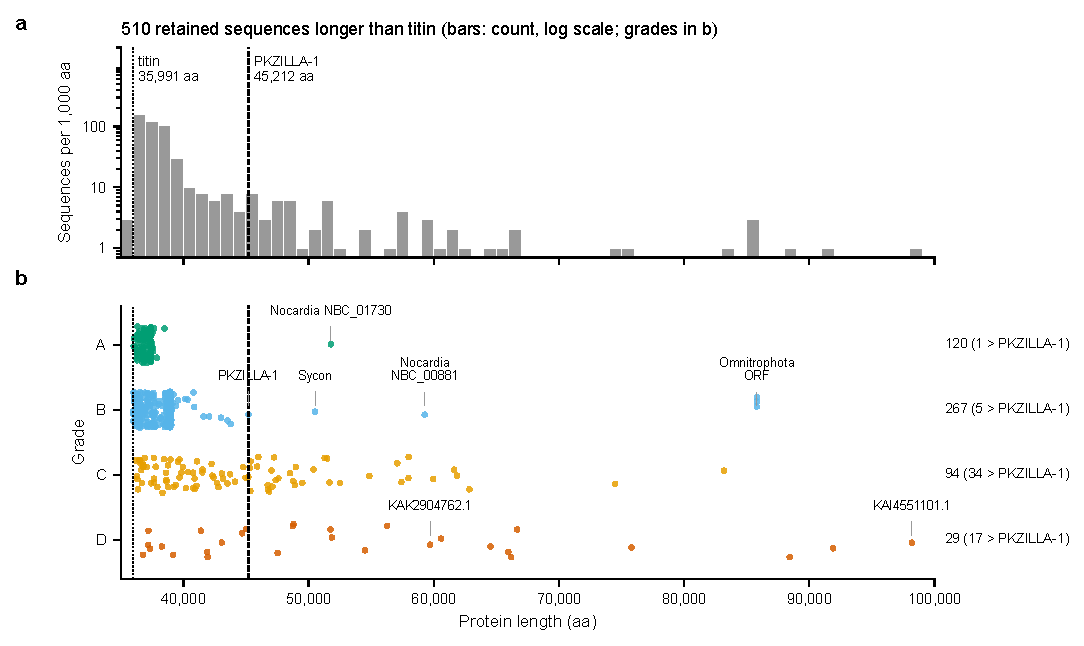
\includegraphics[width=\textwidth]{figures/fig1_lengths_grades.pdf}
\caption{\textbf{Lengths and final grades of the \nm{n_retained} retained sequences.} (a) Sequences per 1,000-aa bin
(log scale). (b) Each sequence as one point by final grade (jittered within a grade). Dotted line: human titin isoform
NP\_001254479.2, \nm{titin_len} aa; dashed line: PKZILLA-1, \nm{pkz_len} aa. Counts give the sequences per grade and
how many are longer than PKZILLA-1. Data: \file{data/locus_checks.tsv}.}
\label{fig:lengths}
\end{figure}

\begin{figure}[t]
\centering
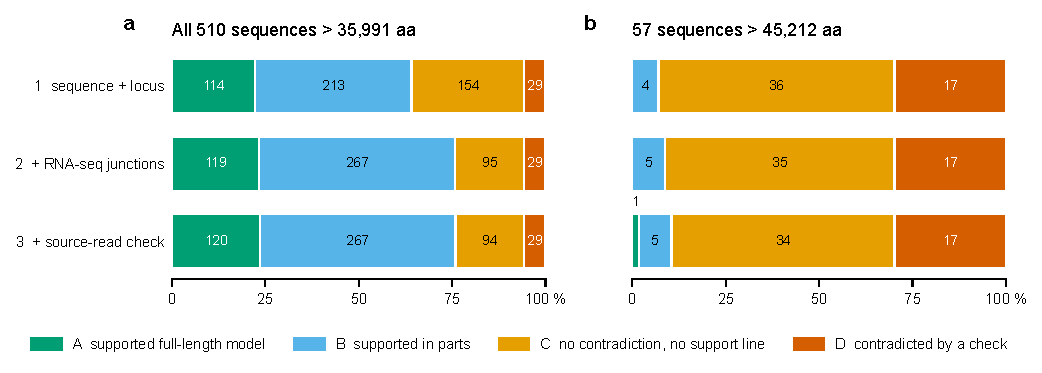
\includegraphics[width=\textwidth]{figures/fig2_grades_by_stage.pdf}
\caption{\textbf{Grades after each evidence stage.} Stage 1: sequence and locus checks; Stage 2: adds RNA-seq junction
evidence for eukaryotic models; Stage 3: adds the source-read check of bacterial assemblies. (a) All \nm{n_retained}
sequences. (b) The \nm{n_retained_gt_pkz} longer than \nm{pkz_len} aa. Data: \file{data/locus_checks.tsv}.}
\label{fig:stages}
\end{figure}

\subsection{Translated tandem repeats: frequent above \nm{pkz_len} aa, but not by themselves a contradiction}

Sequence and locus checks (Stage 1) graded the \nm{n_retained} sequences \nm{s1_all_A}~A, \nm{s1_all_B}~B,
\nm{s1_all_C}~C and \nm{s1_all_D}~D; none of the \nm{n_retained_gt_pkz} longer than \nm{pkz_len} aa reached A
(Figures~\ref{fig:lengths} and~\ref{fig:stages}). The most frequent signal was the translation of a tandem repeat (the D1
pattern): high protein self-identity at the best period, or most residues inside repeated 25-mers, with almost no
recognisable domain. It occurs in \nm{d1_pattern_all} sequences, \nm{d1_pattern_big} of them longer than \nm{pkz_len}
aa (\nm{d1_pattern_big_euk} eukaryotic).

Positive controls showed that this pattern alone does not separate real proteins from questionable models
(Figure~\ref{fig:controls}a; Supplementary Note~2). Among \nm{ctl_n} reviewed proteins with protein-level evidence,
chosen by a rule fixed before scoring, it flagged \nm{ctl_d1_flagged}: three of four complete spidroins, the silk fibroin
heavy chain, four serine-rich bacterial adhesins and two long human proteins. None of the flagged proteins with a coding
sequence showed a DNA-level contradiction. The pattern therefore counts as a contradiction only together with a
non-coding Fickett signal in most coding windows (D2) or several alternative reading frames as open as the annotated one
(D3). Tested on a hold-out set fixed before scoring (\nm{hold_n} further reviewed proteins), the first rule would have
flagged \nm{hold_d1_v1}, the revised rule flagged \nm{hold_d1_v2}. The revision moved \nm{repeat_flag_all} audit sequences
from D to C, \nm{repeat_flag_big} of them longer than \nm{pkz_len} aa. Of the \nm{d1_pattern_big} patterned sequences
above that length, \nm{d_big_d1_with_dna} remain D and \nm{repeat_flag_big} are C with a repeat flag; under the first rule
D would hold \nm{sens_d1v1_big_D} of the \nm{n_retained_gt_pkz}.

\begin{figure}[t]
\centering
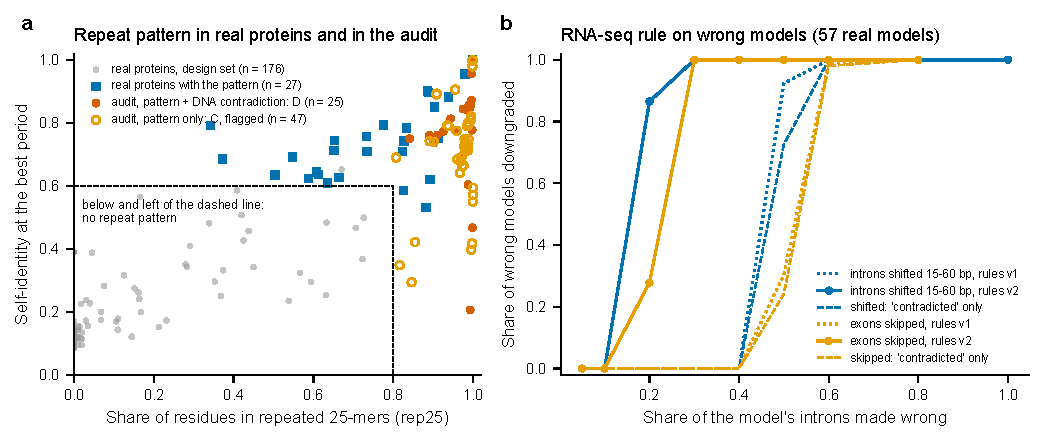
\includegraphics[width=\textwidth]{figures/fig6_controls.pdf}
\caption{\textbf{Controls of the grading rules.} (a) Self-identity at the best period against the share of residues in
repeated 25-mers. Grey: the \nm{ctl_n} real proteins of the design set; blue squares: real proteins with the repeat pattern
(design and hold-out sets); filled circles: audit sequences with the pattern plus a DNA-level contradiction (D); open
circles: audit sequences with the pattern alone (C, repeat flag). The dashed line bounds the pattern. (b) Share of
deliberately wrong versions of \nm{power_models} real models that the RNA-seq rules downgrade, by the share of introns made
wrong; solid: revised verdict order, dotted: first order, dashed: ``contradicted'' alone. Data: \file{controls/d1/},
\file{controls/rna_power/rna_power.tsv}.}
\label{fig:controls}
\end{figure}

The longest retained entry shows the pattern with DNA-level contradiction (Figure~\ref{fig:repeat}). KAI4551101.1
(\nm{ovis_length} aa) from an \spn{Ovis ammon polii} $\times$ \spn{O.~aries} hybrid assembly repeats with a period of
\nm{ovis_protein_period_aa} aa at \nm{ovis_protein_period_identity} identity and has no recognisable domain; its coding
sequence repeats with a period of \nm{ovis_dna_tandem_lag_bp} bp, has a Fickett coding score of \nm{ovis_fickett_median}
(non-coding range), and two alternative frames are nearly free of stop codons. All \nm{ovis_entries} retained entries from
this hybrid share the 22-aa period or a multiple of it and remain D. These models are consistent with open reading frames
called through a GC-rich tandem array; they are not supported as protein-coding genes by the evidence examined
(Supplementary Note~3).

\begin{figure}[t]
\centering
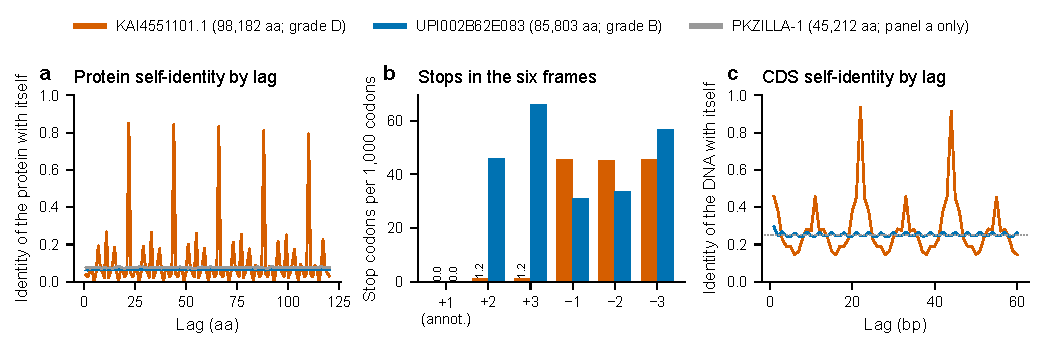
\includegraphics[width=\textwidth]{figures/fig3_tandem_repeat.pdf}
\caption{\textbf{A translated tandem repeat.} (a) Identity of each protein with itself shifted by the given lag.
KAI4551101.1 (grade D) peaks at multiples of 22 aa; the \nm{orf_len_aa}-aa Omnitrophota ORF UPI002B62E083 (grade B)
and PKZILLA-1 stay at background. (b) Stop codons per 1,000 codons in the six reading frames of each coding sequence.
(c) Identity of the coding DNA with itself by lag (first 200 kb). Data: \file{data/fasta/unique_ge35992.fasta.gz},
\file{data/manual/KAI4551101_locus.fa.gz}, \file{data/manual/DAOTDT01.fasta.gz}.}
\label{fig:repeat}
\end{figure}

\subsection{RNA-seq supports most titin-like models but can rarely test the repeat models}

For eukaryotic models we streamed public Illumina RNA-seq runs from ENA and counted spliced reads that match each
annotated intron exactly (Methods); \nm{rna_runs_kept} run results from \nm{rna_species} species were kept. The controls
behaved as expected: human titin had \nm{titin_introns_counted_supported} of \nm{titin_n_introns} introns supported and
none of its \nm{titin_testable_introns} introns with covered flanks unsupported; PKZILLA-1 had all \nm{pkz_n_introns}
supported, \nm{pkz_introns_multi_only} of them only by multi-mapped reads inside repeated modules. Of the
\nm{rna_tested_models} models with a verdict from reads, \nm{rna_full} were ``full'' (at least 90\,\% of introns
supported), \nm{rna_partial} ``partial'' (50--90\,\%), \nm{rna_weak} ``weak'' and \nm{rna_noexpr} without expression in
the runs available; none was ``contradicted''. The stage moved \nm{s1s2_C_to_B} sequences from C to B
(\nm{s1s2_C_to_B_apostichopus} of them isoforms of one \spn{Apostichopus japonicus} gene) and \nm{s1s2_B_to_A} from B to
A. All \nm{s2_all_A} sequences at grade A after this stage are vertebrate titins. Above \nm{pkz_len} aa it added one B:
the sponge \spn{Sycon ciliatum} model XP\_065194412.1 (\nm{sycon_len} aa), with \nm{sycon_introns_unique_support} of
\nm{sycon_n_introns} introns supported by unique reads; its record notes that \nm{sycon_gap_patch_bp} transcript bases
bridge a gap in the genome assembly.

The \nm{rep_models} models that had been graded D under the first repeat rule were tested afterwards, under rules fixed
before the run (Supplementary Note~4, Table~S4). Only \nm{rep_testable} had an assembly and usable runs; the others lack
RNA-seq in ENA (\nm{rep_untestable_noruns}) or a gene model with coordinates (\nm{rep_untestable_nolocus}). Because
multi-mapped reads cannot tell repeat copies apart, these models count only uniquely placed reads, and a correct intron
inside a repeated copy cannot obtain one. In the five testable models longer than \nm{pkz_len} aa, at most
\nm{mapp_syn1_pct}\,\% of introns have a junction sequence that is unique within the model, so ``partial'' support was out
of reach before any read was counted. The results fit this: the two \spn{Schistosoma haematobium} isoform models were
``partial'' (\nm{rep_schisto1_supported} of \nm{rep_schisto1_introns} and \nm{rep_schisto2_introns} introns, none
unsupported among \nm{rep_schisto1_testable} testable ones) and move from C to B; \spn{Owenia} and \spn{Arctogadus} models
were ``weak''; the six stickleback, eel and \spn{Acnodon} models had at most \nm{rep_noexpr_max_unique} uniquely placed
reads. No model was contradicted, and no grade above \nm{pkz_len} aa changed. One test run of a \spn{Schistosoma} model
was seen before the rules were committed; the rule code predates it, and its result is not needed for the verdict
(Supplementary Note~4).

\subsection{Two fish titin models are consistent with merged tandem titin genes}

Zebrafish has two titin genes in tandem, \gene{ttna} and \gene{ttnb} \citep{seeley2007}. KAK2904762.1
(\spn{Cirrhinus molitorella}, \nm{cirrhinus_len} aa, \nm{cirrhinus_exons} exons) splits into two titins
(Figure~\ref{fig:fish}): positions 1--\nm{cirrhinus_first_end} follow zebrafish \gene{ttna} from its N- to its C-terminus
(\nm{cirrhinus_first_ttna} windows), and from position \nm{cirrhinus_second_copy_start_aa} the windows start again at a
titin N-terminus and run to the C-terminus of \gene{ttnb} (\nm{cirrhinus_second_ttnb}). Across \nm{cirrhinus_runs}
RNA-seq runs, the intron at amino acid \nm{cirrhinus_join_intron_aa}, right after the \gene{ttna}-like C-terminus, has no
junction read, while the five introns before it have a median of \nm{cirrhinus_join_before_median} reads and the five
after it \nm{cirrhinus_join_after_median}. TSR51413.1 (\spn{Bagarius yarrelli}, \nm{bagarius_len} aa) shows the same
two-part pattern, with too few reads to test the join. Both were graded D5 (parts of different complete proteins). We
describe them as consistent with two adjacent titin genes joined in one model; gene order on the source contigs was not
checked independently.

\begin{figure}[t]
\centering
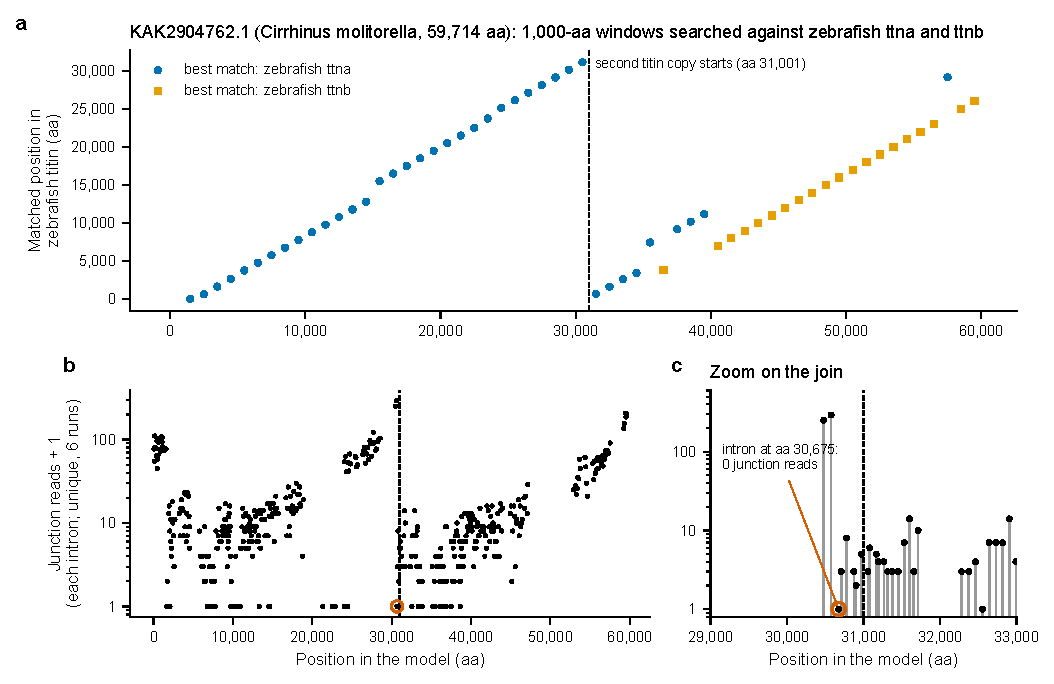
\includegraphics[width=\textwidth]{figures/fig4_fish_titin_pair.pdf}
\caption{\textbf{A model consistent with two merged titin genes.} (a) KAK2904762.1 in 1,000-aa windows searched
against zebrafish ttna (circles) and ttnb (squares); y is the start of the best match. The match restarts at a titin
N-terminus at aa \nm{cirrhinus_second_copy_start_aa} (dashed line). (b) Uniquely mapped junction reads per intron,
summed over \nm{cirrhinus_runs} runs (reads + 1). (c) The join: the intron at aa \nm{cirrhinus_join_intron_aa} (open
circle) has no junction read. Data: \file{data/followups/fish_titin_pair.tsv}, \file{data/rnaseq_run_results.tar.gz}.}
\label{fig:fish}
\end{figure}

\subsection{Source reads support the bacterial giants, with one untestable repeat}

Bacterial models cannot be tested with RNA-seq, because no strain-level transcript data exist for these organisms. For
the \nm{orf_len_aa}-aa Omnitrophota open reading frame (three assemblies) and two \spn{Nocardia} models on complete
genomes, we re-mapped all reads used to build each assembly and checked depth, read-pair continuity, clipped reads,
discordant pairs and the reading frame of the read consensus, with an artificial misassembly as a negative control in
every run (Methods; Supplementary Note~3).

Both \spn{Nocardia} models are supported by Illumina and nanopore reads (median unique depth \nm{dna_nbc01730_depth} and
\nm{dna_nbc00881_depth}, gene-to-contig depth ratio \nm{dna_nbc01730_ratio}). With an orthologue of consistent length,
WP\_327112628.1 (\nm{nbc01730_len} aa) reaches A; WP\_406270362.1 (\nm{nbc00881_len} aa) reaches B, because the same
homologue gives it a length ratio of \nm{nbc00881_ratio}. Neither has transcript or peptide evidence; for these bacteria,
A means that the gene model is supported by the assembly, its reads and orthology, not that the protein is made.

A single \nm{orf_bp}-bp open reading frame of \nm{orf_len_aa} aa occurs in three metagenome-assembled genomes from three
samples (DAOTDT01, DAOPMG01, DAOOUB01), \nm{omni_aa_identity_min_pct}--\nm{omni_aa_identity_max_pct}\,\% identical
(Figure~\ref{fig:omni}). Over the gene, the reads of each sample give median unique depths of \nm{dna_tdt_depth},
\nm{dna_pmg_depth} and \nm{dna_oub_depth}, at most \nm{dna_tdt_discordant_pct}\,\% discordant pairs per window, and no
frame-breaking change. The gene carries a direct repeat: two copies of about \nm{rep_copy_bp_kb} kb,
\nm{rep_lag_bp} bp apart, that differ at \nm{rep_diffs} positions in all three assemblies. Fragments of these libraries
cannot be placed uniquely inside a copy, so the middle of each copy cannot be tested; a first version of our check
mistook this for a break, and the revised check asks how many spanning pairs a correct assembly would give before
counting a missing pair against it. Two assemblies are ``supported outside 1.3 kb of repeat'' and the third is
``inconclusive'' at one boundary at the edge of a copy (\nm{dna_oub_weakest_obs} pairs where about
\nm{dna_oub_weakest_exp} are expected). The locus stays at B; whether the copies are joined in the assembled order cannot be
decided with these libraries, and no long-read data exist for these samples.

\begin{figure}[t]
\centering
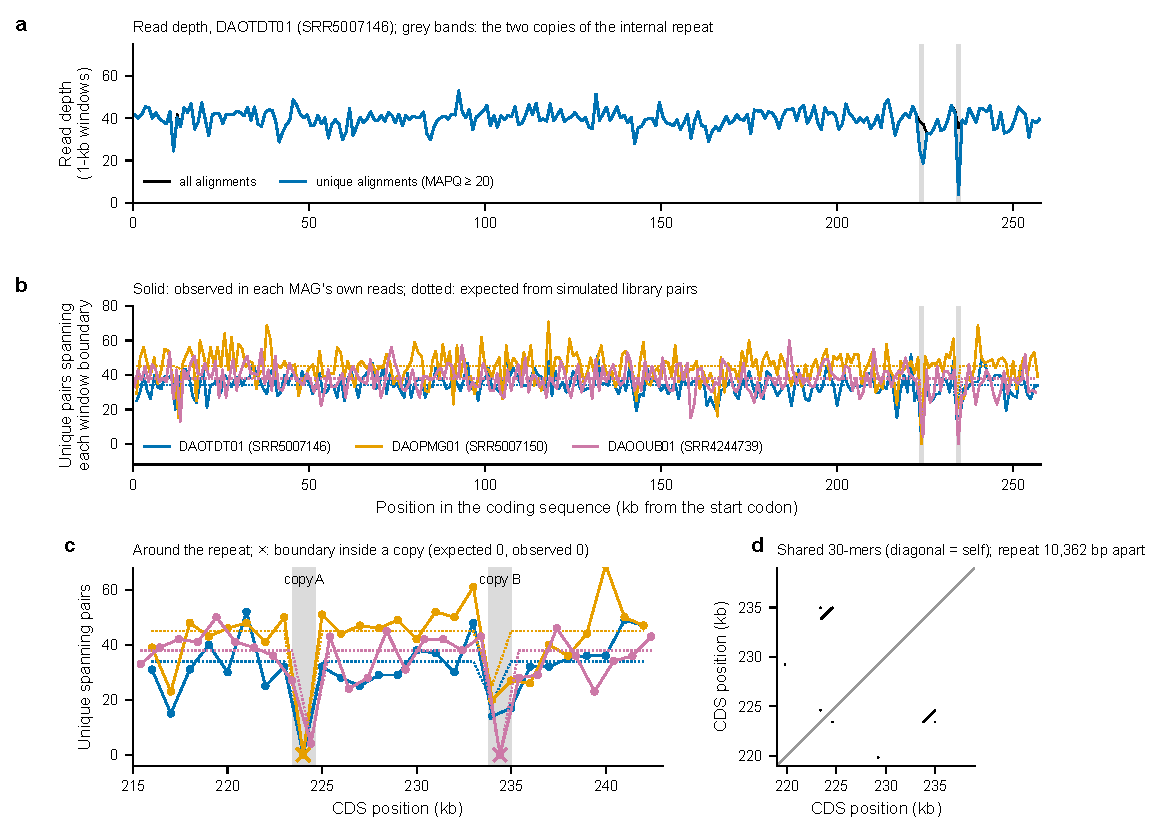
\includegraphics[width=\textwidth]{figures/fig5_omnitrophota_orf.pdf}
\caption{\textbf{Source-read check of the \nm{orf_len_aa}-aa Omnitrophota ORF.} (a) Read depth per 1-kb window in
DAOTDT01: all alignments and uniquely placed alignments (MAPQ $\geq$ 20); unique depth drops only at the two repeat
copies (grey bands). (b) Uniquely placed read pairs spanning each 1-kb boundary in each assembly's own reads (solid) and
the number expected from simulated pairs of the same library (dotted). (c) The repeat; $\times$ marks boundaries inside a
copy, where 0 pairs are expected and 0 were observed. (d) Shared 30-mers within the coding sequence from 219 to 239 kb.
Data: \file{data/dna_checks/*.json}, \file{data/manual/DAOTDT01.fasta.gz}.}
\label{fig:omni}
\end{figure}

\subsection{Peptides cover only the N-terminal part of a \texorpdfstring{\nm{prot_giant_len}}{39,686}-aa bacterial protein}

WP\_128698900.1 of \Ca{} Velamenicoccus archaeovorus (\nm{prot_giant_len} aa) is shorter than PKZILLA-1, but its organism
has a public proteomics dataset, PRIDE PXD025008 \citep{kizina2022}. The dataset's authors list ``a very large multienzyme
surface protein (4,384~kDa)'' among the most frequently detected proteins, whose ``gene codes for 39,678 amino acids''
\citep{kizina2022}. Our analysis confirms their detection and maps where the peptides fall.

We first searched the authors' deposited peak lists and then, because those turned out to hold only
\nm{raw_mgf_share_pct}\,\% of the MS/MS spectra, all \nm{raw_files} raw files (\nm{raw_ms2} spectra) with Sage
\citep{lazear2023}, against the authors' database with the organism's earlier protein set replaced by the proteins of its
closed genome, plus a reversed and a shuffled copy of the giant (Methods; Supplementary Note~5, Table~S5). In the raw
files, \nm{raw_giant_peptides} peptides unique to WP\_128698900.1 passed 1\,\% FDR at the spectrum, peptide and protein
levels (\nm{raw_giant_psms} PSMs). \nm{raw_giant_first6000} of them start within the first 6,000 aa; three lie further
on, at aa \nm{raw_giant_after6000}, each from a single spectrum; none maps after residue \nm{raw_giant_last_end}
(\nm{raw_giant_last_pct}\,\% of the length; Figure~\ref{fig:peptides}). The gap is not a property of the sequence: fully
tryptic peptides of 7--40 aa occur evenly along it (\nm{prot_tryptic_range} per 1,000 aa), and no peptide lies inside or
after the protein's internal repeat blocks (aa \nm{prot_repeat_span}). The reversed and shuffled copies obtained no PSM
at 1\,\% FDR, while elongation factor Tu of the same organism was covered to \nm{raw_eftu_cov_pct}\,\% by
\nm{raw_eftu_peptides} unique peptides. The peak-list search gave the same picture (\nm{prot_giant_peptides} peptides,
\nm{raw_both} shared with the raw-file search); its one peptide beyond residue 16,000 (start \nm{raw_mgf_only_after6000}, peptide
$q = $ \nm{prot_peak_last_q}) was not found in the raw files.

These peptides show that the N-terminal part of the protein is made. They do not show that a single
\nm{prot_giant_len}-aa chain is made, and their absence from the C-terminal \nm{raw_giant_unc_pct}\,\% neither supports nor rules out that part
of the model. The entry stays at C: our peptide line requires unique peptides in all five fifths of the length, and the
raw-file search covers two. That line was written after this result had been seen; a first draft that asked for three
fifths would have counted the peak-list search as support (Supplementary Note~1).

For the \nm{sycon_len}-aa \spn{Sycon ciliatum} model we examined the two PRIDE projects listed for the species. PXD031991 holds
acid-extracted, chemically derivatised histones \citep{graubove2022} and is not suited to detecting this protein.
PXD060105 is a proteome of the spicule organic matrix \citep{voigt2025}; the authors' search database contains the model's
sequence as \nm{sy_fragments} transcript-derived fragments, and their report of \nm{sy_authors_n} proteins does not
include it. In our search of the \nm{sy_raw_files} raw files, no spectrum matched the model at 1\,\% spectrum-level FDR,
while \nm{sy_authors_found} of the authors' \nm{sy_authors_n} proteins were recovered; the dataset is too small to reach
1\,\% at peptide or protein level for any protein. A giant protein is not expected in a mineral matrix prepared by
dissolving the surrounding tissue, so this absence says nothing about the model.

\begin{figure}[t]
\centering
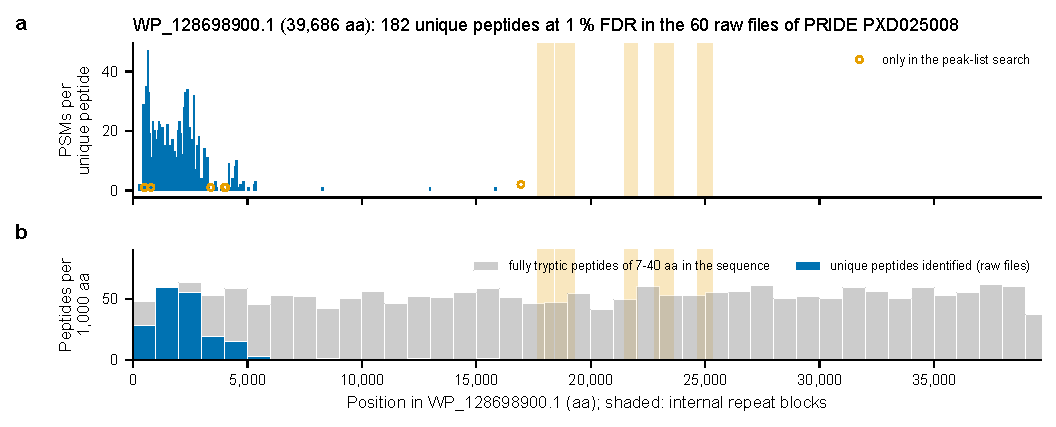
\includegraphics[width=\textwidth]{figures/fig7_peptides.pdf}
\caption{\textbf{Peptides of WP\_128698900.1 in PRIDE PXD025008.} (a) Each peptide unique to the protein at 1\,\% FDR
(spectrum, peptide and protein level) in the search of all \nm{raw_files} raw files, at its start position; height is
its number of PSMs. Open circles: peptides found only in the search of the deposited peak lists. (b) Per 1,000 aa: unique
peptides identified in the raw files (blue) and fully tryptic peptides of 7--40 aa in the sequence (grey). Shaded:
internal repeat blocks (20-mers occurring more than once, blocks of at least 100 aa). Data:
\file{proteomics/results/raw60_giant_peptides.tsv}, \file{proteomics/results/full6_giant_peptides.tsv},
\file{proteomics/results/verify_extra.json}.}
\label{fig:peptides}
\end{figure}

\subsection{What remains above \nm{pkz_len} aa}

After all stages, the \nm{n_retained} sequences grade \nm{fin_all_A}~A, \nm{fin_all_B}~B, \nm{fin_all_C}~C and
\nm{fin_all_D}~D. In the leaderboard (Supplementary Table~S1), isoforms of one gene, near-identical copies in several
assemblies and duplicate records of one gene in one genome (\nm{lb_merged_records} records merged) form one row each,
giving \nm{lb_loci} graded loci: \nm{lb_A}~A, \nm{lb_B}~B, \nm{lb_C}~C and \nm{lb_D}~D. Above \nm{pkz_len} aa there are
\nm{lb_big} loci: \nm{lb_big_A}~A, \nm{lb_big_B}~B, \nm{lb_big_C}~C and \nm{lb_big_D}~D (Table~\ref{tab:candidates}).
Grade A is otherwise reached only by \nm{lb_A_titin_loci} vertebrate titin loci (\nm{lb_A_titin_min}--\nm{lb_A_titin_max}
aa). The A/B status of the four loci in Table~\ref{tab:candidates} held in \nm{sens_big_ab_stable} of \nm{sens_variants}
threshold settings; the exceptions were counting a single open alternative frame as D3 and requiring 10 junction reads per
intron (Supplementary Table~S3).

\begin{table}[t]
\centering\small
\caption{Loci longer than \nm{pkz_len} aa graded A or B.}\label{tab:candidates}
\begin{tabularx}{\textwidth}{L{2.6cm} L{2.4cm} r c Y Y}
\toprule
Accession & Organism & Length (aa) & Grade & Supported by & Missing \\
\midrule
UPI002B62E083 (+2 copies) & \Ca{} Omnitrophota (3 MAGs) & \nm{orf_len_aa} & B & one ORF in 3 assemblies; coding signal; source
reads outside a 1.2-kb repeat & long reads across the repeat; orthologue; expression or peptides \\
WP\_406270362.1 & \spn{Nocardia} sp.\ NBC\_00881 & \nm{nbc00881_len} & B & complete genome; coding signal; Illumina and
nanopore reads & orthologue of consistent length (ratio \nm{nbc00881_ratio}); expression; peptides \\
WP\_327112628.1 & \spn{Nocardia} sp.\ NBC\_01730 & \nm{nbc01730_len} & A & complete genome; coding signal; Illumina and
nanopore reads; homologue of \nm{nbc01730_best_len} aa & expression; peptides \\
XP\_065194412.1 & \spn{Sycon ciliatum} & \nm{sycon_len} & B & RNA-seq: \nm{sycon_introns_unique_support} of
\nm{sycon_n_introns} introns, full CDS coverage & orthologue (closest \nm{sycon_best_homolog_len} aa); bridges a
\nm{sycon_gap_patch_bp}-bp assembly gap with transcript sequence; peptides \\
\bottomrule
\end{tabularx}
\end{table}

\section{Discussion}

The longest entries in protein databases are mostly not supported as full-length gene models by the evidence we
examined. Of the \nm{n_retained_gt_pkz} sequences longer than PKZILLA-1, \nm{fin_big_D} are contradicted by at least one
check, \nm{fin_big_C} have no line of support (\nm{repeat_flag_big} of them with the repeat pattern), and six, at four loci,
are supported as gene models.

The most frequent pattern is a protein that reads like the translation of a tandem DNA repeat. Our controls show that the
pattern is not, by itself, evidence against a model: real silk proteins and serine-rich adhesins share it, and at the
protein level nothing we measured separates them from the audit entries. The difference lies in the coding sequence:
\nm{d_big_d1_with_dna} of the patterned entries above \nm{pkz_len} aa have a non-coding DNA signal or several open frames,
which none of the real proteins with a coding sequence showed. The other \nm{repeat_flag_big} remain unresolved:
\nm{flag_big_weak_coding} have a weak coding signal (Fickett median \nm{flag_big_weak_coding_range}), which is absence
of support rather than a contradiction, \nm{flag_big_coding} look like real repetitive genes by every sequence test, and
\nm{flag_big_nodna} have no locus that could be tested. Short-read RNA-seq is a weak tool for them: in a tandem array a
junction read fits every copy, so the test can show that the unique parts are spliced as annotated, but not how many
copies the gene has. Long-read transcripts spanning the array, or peptides along the whole model, would decide them.

The merging of neighbouring genes, here two titin paralogues, is harder to detect without a reference proteome or
transcript evidence; junction reads across the join gave a clear signal in one of the two cases. The remaining candidates
are bacterial or sponge models, supported at the level of the gene model: assemblies, reads, coding signal and, for one
\spn{Nocardia} model, orthology. None has protein-level evidence: PRIDE lists no project for the Omnitrophota or
\spn{Nocardia} organisms by species name, and the one \spn{Sycon} proteome suitable for a search is of a fraction where the
protein would not be expected. By contrast, PKZILLA-1 itself has published peptide support \citep{fallon2024}. The
\nm{orf_len_aa}-aa Omnitrophota ORF falls in the length class reported by \citet{westroberts2023} for curated
Omnitrophota genomes; we could not compare sequences, because their data repository was not reachable from our
environment. Our observation adds read-level support from the three source metagenomes and identifies the one stretch that
short reads cannot resolve.

The one positive proteomic case shows what peptides can and cannot settle. For the \nm{prot_giant_len}-aa
\spn{Velamenicoccus} protein they confirm that the N-terminal part is made, as its authors reported \citep{kizina2022},
in the full raw data as in the deposited peak lists. They say nothing about the C-terminal \nm{raw_giant_unc_pct}\,\%, although tryptic
peptides are as dense there as elsewhere. That absence is weak evidence either way: the model could be wrong beyond that
point, or the C-terminal part could be cleaved off or harder to extract or detect. A grade based on peptides should
therefore require them along the whole model.

The table also says what would change each grade. For the repeat models, long-read transcripts that span the whole array
would show whether the copies are spliced into one messenger RNA, and peptides from the repeat-flanking regions would show
whether the protein continues past them. For the Omnitrophota ORF, long reads or long-insert libraries from the same
samples would settle the arrangement of the repeat copies. For the \spn{Sycon} model, a proteome of whole tissue searched
against the full model, rather than a mineral fraction, would test whether the gene is translated. For the
\spn{Velamenicoccus} protein, the open question is the C-terminal \nm{raw_giant_unc_pct}\,\%: a targeted search for its peptides, or a
proteome of a fraction enriched for surface proteins, could show whether it is part of the same chain. The column
\file{still_missing} of Supplementary Table~S1 lists this per locus.

A grade records which checks a model passed with the data available on the snapshot dates. It is not a statement about
the biology of the gene, does not assess the work of the submitters, and should be updated as new assemblies, transcripts
or peptides appear.

\subsection*{Limitations}
\begin{enumerate}[leftmargin=*]
\item \textbf{The rules are ours.} They were set on two controls and revised seven times during the work, three times
after controls had been run; only the repeat rule was retested on an independent set, and one support line (peptides) was
written after its only test case had been seen. All revisions and their effects are in Supplementary Note~1.
\item \textbf{RNA-seq is incomplete and uneven.} Runs were taken from whatever tissues ENA offered; \nm{rna_runs_stream_error}
runs ended early on a dropped connection, so junction counts are lower bounds, and a ``weak'' or ``no-expression''
verdict is not evidence against a model. Repeat models can be tested only where their junctions are unique, and the
power test shows that errors in fewer than 30\,\% of introns are often missed (Supplementary Notes~2 and~4).
\item \textbf{Little protein evidence.} Two proteomic datasets were searched and a third examined; the only peptides
found concern an entry shorter than \nm{pkz_len} aa. Our search limits (one missed cleavage, peptides of 7--40 aa) were set to fit a
laptop's memory. Peptides show that parts of a protein are made, not that it is made as one chain.
\item \textbf{Repeats limit what short reads can test.} The 1.2-kb Omnitrophota repeat cannot be crossed by the
available libraries, and our copy-number test cannot see an error shorter than 3 kb there; the three assemblies come from
one study and one pipeline.
\item \textbf{Scope.} MGnify and other metagenomic catalogues were not included; most bacterial entries rest on sequence
and assembly checks only; orthology was judged by length consistency of DIAMOND hits in UniProtKB, which favours
well-sampled clades; every count refers to the stated snapshot dates.
\end{enumerate}
Supplementary Note~6 lists these limitations in full.

\section{Methods}

Full methods, with every threshold, are in Supplementary Methods; code paths are given there.

\paragraph{Inventory.} UniProtKB (release 2026\_04) and UniParc were queried through the UniProt REST API
\citep{uniprot2025}, and NCBI Protein with the Entrez length filter \texttt{35992:100000000[SLEN]} on 11 November 2026
\citep{sayers2026,oleary2016}. Sequences were merged by MD5 checksum; withdrawn, patent or synthetic records and titles
marked ``partial'' were excluded; loci were defined by shared NCBI GeneID or overlapping coordinates. All requests used a
generic user agent within the providers' anonymous rate limits.

\paragraph{Stage 1: sequence and locus checks.} For each protein we computed low-complexity and X content, the share of
residues in repeated 25-mers, the best tandem period and its self-identity, and coverage by a panel of \nm{hmm_panel}
Pfam profile HMMs \citep{mistry2021} searched with PyHMMER \citep{eddy2011,larralde2023}. Locus DNA was fetched from
INSDC/RefSeq to measure exon structure, distance to contig ends, N runs, GC by codon position, the Fickett statistic in
300-bp windows \citep{fickett1982}, stop codons in the alternative frames and the DNA tandem period. Proteins were cut into
1,000-aa windows and searched with DIAMOND 2.2.8 \citep{buchfink2021} against UniProtKB for orthologues and fusions.
Contradiction rules (D1 repeat pattern, only with D2 or D3; D2 non-coding Fickett signal; D3 open alternative frames;
D4 Ns or joins across contigs; D5 parts of different complete proteins) and support lines (S1 orthologue of consistent
length; S2 near-identical copy in another assembly; S3 NCBI report of full RNA-seq support; S4 curated RefSeq record;
S6 unique peptides in all five fifths of the length) define the grades as in Table~\ref{tab:grades}. Record twins of one
genome (RefSeq and GenBank or UniProtKB copies) do not count as independent.

\paragraph{Stage 2: RNA-seq.} For eukaryotic models at grade B or C, four to six public Illumina RNA-seq runs per
species (0.2--6~GB, not single-cell, different studies first, muscle first for titin-like models) were read from ENA
\citep{yuan2026}, at most 60 million reads per file; runs first cut short by a read-saturation rule were repeated without
it. Reads were filtered
with minimap2 2.31 \citep{li2018} against the coding exons and aligned with \texttt{-x splice:sr} to the whole genome,
which serves as a decoy; alignments were handled with samtools \citep{danecek2021}. An intron is supported by at least
three exactly matching reads; multi-mapped reads count only for models without a repeat flag. An intron is testable when
both flanking exons reach a mean unique depth of 10 in one run. Verdicts, in order: no-expression ($<$ 50 unique reads);
contradicted ($\geq$ 10 testable introns with $\geq$ 50\,\% unsupported, or more reads on junctions leaving the gene than
on annotated ones); under-supported where covered ($\geq$ 20\,\% of $\geq$ 10 testable introns unsupported); full
($\geq$ 90\,\% supported); partial ($\geq$ 50\,\%); otherwise weak. For the repeat-flag stage, files were downloaded to
disk with resumed retries before mapping, and a contradiction had to hold also on introns whose junction is unique within
the model (\file{cloud/bundle_rep_rna/RULES.txt}).

\paragraph{Stage 3: source reads.} Illumina pairs and nanopore reads from each assembly's BioSample were mapped with
minimap2 to the whole assembly. In 1-kb windows over the gene we measured unique and total depth, uniquely placed pairs
spanning each boundary, clip pile-ups, discordant pairs, the gene-to-contig depth ratio and frame-breaking consensus
changes. A boundary is tested only where simulated error-free pairs of the same library would give at least five unique
spanning pairs; stretches below that must be crossed as a whole. Since version 3.1 a copy-number test flags at least three
consecutive windows whose total depth departs from the gene's depth by more than a factor of $\sqrt{2}$. Every check ran a
negative control with an inverted join at the gene midpoint.

\paragraph{Proteomics.} For PXD025008 the authors' database was kept, minus their reversed entries and with the
organism's earlier genome-bin proteins replaced by the GenBank translations of its closed genome (CP019384.1); QAT16263.1
was replaced by its RefSeq version WP\_128698900.1. For PXD060105, database entries of which at least half of the 10-mers
occur in XP\_065194412.1 were treated as fragments of the same gene and replaced by the full model. Raw files were
converted with ThermoRawFileParser \citep{hulstaert2020} (vendor peak picking) and
searched with Sage 0.14.7 \citep{lazear2023}: trypsin, one missed cleavage, peptides of 7--40 aa, 10 ppm precursor
tolerance, fragment tolerance 0.5 Da (ion trap) or 20 ppm (Orbitrap), variable methionine oxidation, fixed
carbamidomethylation only where the authors used it, reversed decoys. Identifications were kept at spectrum, peptide and
protein $q \leq 0.01$; a peptide is unique if its sequence (I = L) occurs in no other entry of the database. Each database
replaced partial or earlier versions of the model by the full model and added a reversed and a shuffled copy as controls.

\paragraph{Controls and sensitivity.} The repeat-rule design and hold-out sets were defined by UniProtKB queries fixed
before scoring. The RNA-seq power test scored deliberately wrong versions of \nm{power_models} real models (introns
shifted by 15--60 bp or exons removed, \nm{power_reps} repeats per setting) against the stored junction counts. Known
misassemblies were built from the finished \spn{Nocardia} sp.\ NBC\_01730 genome and checked with its own reads.
Thresholds were varied one at a time by rerunning the pipeline in a copy of the repository; the published setting
reproduced the released grades exactly.

\paragraph{Numbers and figures.} Every number in this manuscript is printed from \file{paper/numbers.tex}, which
\file{paper/make_numbers.py} computes from the repository's files; \file{paper/NUMBERS.md} maps the text to its sources.
Figures were drawn with matplotlib by \file{paper/make_figures.py}.

\section*{Data and code availability}
All scripts, intermediate tables, per-run RNA-seq results, source-read check results, proteomics results and the code
that computes the numbers, tables and figures of this manuscript are public at
\url{https://github.com/papexlabs/giant-proteins} (code under the MIT licence, data under CC BY 4.0) and archived at
Zenodo (\url{https://doi.org/10.5281/zenodo.24201672}). Every input is public and identified by accession in Supplementary Table~S1 and
the data files. Large inputs (reads, raw spectra, genomes) are downloaded by the scripts and listed with their sizes in
the repository's data manifest.

\section*{Statements}
\noindent\textbf{Author contributions.} A.T.M. is the sole author. He chose the question, set the scope and the
budget, approved each stage before it ran, decided which additional controls and analyses to run and which claims to
keep or withdraw, and reviewed the manuscript. He is responsible for its content.\\[4pt]
\textbf{Use of AI tools.} Most of the hands-on work in this study was done by an AI system under the author's
direction: Claude (Anthropic; model Claude Fable 5.2), used through the Claude Code command-line tool between 11 and
13 November 2026. The AI system searched the literature and the databases, wrote all analysis code, ran it on a
laptop and on rented cloud machines, proposed the grading rules and their revisions, drew the figures, compiled the
tables and wrote the first draft of this text, which the author then reviewed and edited. The author did not write
the code and did not recompute the results by hand. For that reason every number in the text is printed directly
from the data files by a script, every rule change is listed in Supplementary Note~1, and the repository reproduces
the grades from the stored results. An AI system cannot take responsibility for a paper and is not an author; errors
are the author's responsibility.\\[4pt]
\textbf{Competing interests.} A.T.M. is the founder of Papex Labs, which runs papex.org, a service for recording
research provenance. He has no financial interest in any protein, database or sequencing product discussed here.\\[4pt]
\textbf{Funding.} This work received no external funding. Cloud computing (about US\$5) was paid for by Papex
Labs.\\[4pt]
\textbf{Acknowledgements.} This study depends entirely on open resources: UniProt, NCBI (Protein, RefSeq, GenBank,
SRA), the European Nucleotide Archive, PRIDE and Pfam, and on the researchers who deposited the assemblies, reads and
spectra reused here.

\bibliographystyle{unsrtnat}
\bibliography{refs}
\end{document}
